\begin{figure*}[!ht]
  \centering
  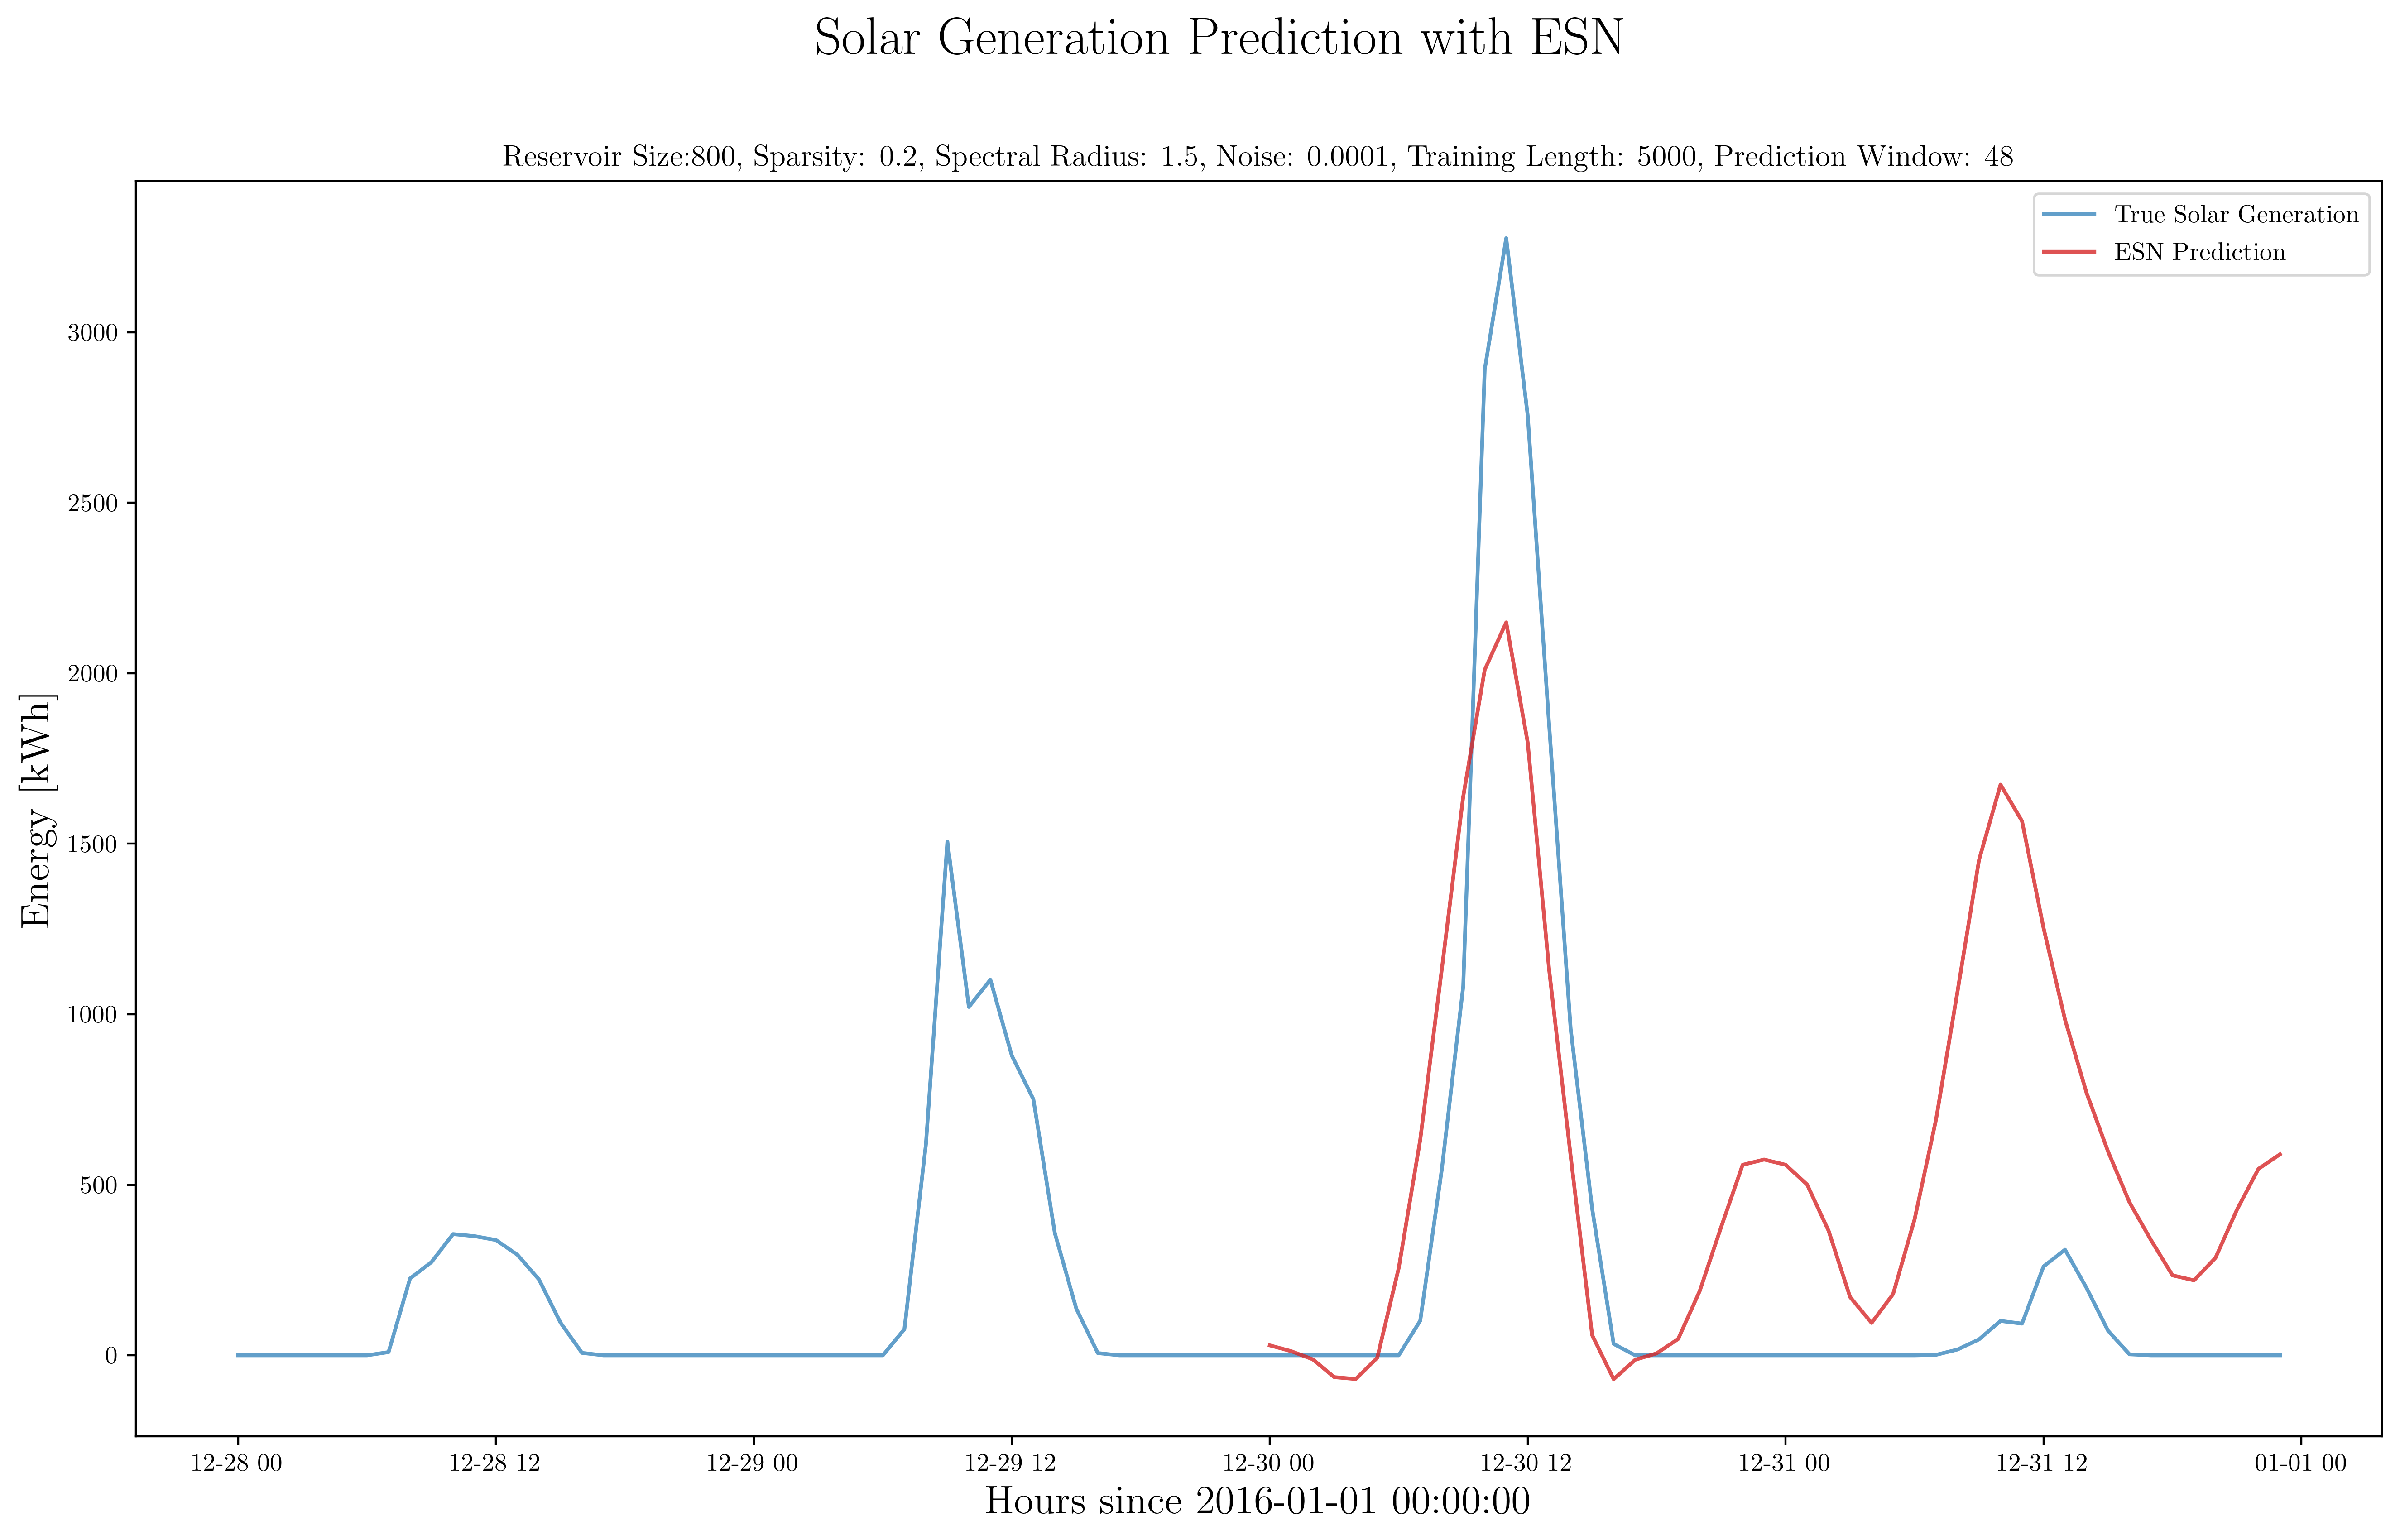
\includegraphics[width=0.8\textwidth]{48_solar_humidity_prediction.png}
  \caption{The optimized 48-hour ahead solar energy prediction with humidity as a  meteorological
  predictor.}
  \label{fig:solar48}
\end{figure*}
% \begin{center}
  \begin{table*}[!ht]
    \centering
    \caption{Tabulated error for 48-hour ahead solar energy forecasts with various coupled quantities. Improvement indicates the percentage improvement over the base case of forecasting solar energy alone.}
    \label{tab:solar48}
    \begin{tabular}{l|c|c|c|c}
      &  & & Improvement & Improvement \\
      Scenario  & MAE & RMSE & MAE (\%) & RMSE (\%)\\
      \hline
      Solar Energy & 0.143276 & 0.206162 & [-] & [-] \\
      Solar + Sun Elevation & 0.200627 & 0.292516 & +40.02 & +41.88\\
      Solar + Humidity & 0.086920 & 0.111476 & -39.33& -45.93\\
      Solar + Pressure & 0.098554 & 0.152672 &-31.21& -25.94\\
      Solar + Wet Bulb Temp. & 0.114157 & 0.167503 & -20.32& -18.75\\
      Solar + Dry Bulb Temp. & 0.079036 & 0.123783 & -44.84& -39.96\\
      Solar + Wind Speed & 0.147270 & 0.191722 & +2.788& -7.004\\
    \end{tabular}
  \end{table*}
% \end{center}
